\documentclass[journal,12pt,twocolumn]{IEEEtran}

\usepackage{setspace}
\usepackage{gensymb}

\singlespacing


\usepackage[cmex10]{amsmath}

\usepackage{amsthm}

\usepackage{mathrsfs}
\usepackage{txfonts}
\usepackage{stfloats}
\usepackage{bm}
\usepackage{cite}
\usepackage{cases}
\usepackage{subfig}

\usepackage{longtable}
\usepackage{multirow}

\usepackage{enumitem}
\usepackage{mathtools}
\usepackage{steinmetz}
\usepackage{tikz}
\usepackage{circuitikz}
\usepackage{verbatim}
\usepackage{tfrupee}
\usepackage[breaklinks=true]{hyperref}
\usepackage{graphicx}
\usepackage{tkz-euclide}

\usetikzlibrary{calc,math}
\usepackage{listings}
    \usepackage{color}                                            %%
    \usepackage{array}                                            %%
    \usepackage{longtable}                                        %%
    \usepackage{calc}                                             %%
    \usepackage{multirow}                                         %%
    \usepackage{hhline}                                           %%
    \usepackage{ifthen}                                           %%
    \usepackage{lscape}     
\usepackage{multicol}
\usepackage{chngcntr}

\DeclareMathOperator*{\Res}{Res}

\renewcommand\thesection{\arabic{section}}
\renewcommand\thesubsection{\thesection.\arabic{subsection}}
\renewcommand\thesubsubsection{\thesubsection.\arabic{subsubsection}}

\renewcommand\thesectiondis{\arabic{section}}
\renewcommand\thesubsectiondis{\thesectiondis.\arabic{subsection}}
\renewcommand\thesubsubsectiondis{\thesubsectiondis.\arabic{subsubsection}}


\hyphenation{op-tical net-works semi-conduc-tor}
\def\inputGnumericTable{}                                 %%

\lstset{
%language=C,
frame=single, 
breaklines=true,
columns=fullflexible
}
\begin{document}


\newtheorem{theorem}{Theorem}[section]
\newtheorem{problem}{Problem}
\newtheorem{proposition}{Proposition}[section]
\newtheorem{lemma}{Lemma}[section]
\newtheorem{corollary}[theorem]{Corollary}
\newtheorem{example}{Example}[section]
\newtheorem{definition}[problem]{Definition}

\newcommand{\BEQA}{\begin{eqnarray}}
\newcommand{\EEQA}{\end{eqnarray}}
\newcommand{\define}{\stackrel{\triangle}{=}}
\bibliographystyle{IEEEtran}
\providecommand{\mbf}{\mathbf}
\providecommand{\pr}[1]{\ensuremath{\Pr\left(#1\right)}}
\providecommand{\qfunc}[1]{\ensuremath{Q\left(#1\right)}}
\providecommand{\sbrak}[1]{\ensuremath{{}\left[#1\right]}}
\providecommand{\lsbrak}[1]{\ensuremath{{}\left[#1\right.}}
\providecommand{\rsbrak}[1]{\ensuremath{{}\left.#1\right]}}
\providecommand{\brak}[1]{\ensuremath{\left(#1\right)}}
\providecommand{\lbrak}[1]{\ensuremath{\left(#1\right.}}
\providecommand{\rbrak}[1]{\ensuremath{\left.#1\right)}}
\providecommand{\cbrak}[1]{\ensuremath{\left\{#1\right\}}}
\providecommand{\lcbrak}[1]{\ensuremath{\left\{#1\right.}}
\providecommand{\rcbrak}[1]{\ensuremath{\left.#1\right\}}}
\theoremstyle{remark}
\newtheorem{rem}{Remark}
\newcommand{\sgn}{\mathop{\mathrm{sgn}}}
\providecommand{\abs}[1]{\left\vert#1\right\vert}
\providecommand{\res}[1]{\Res\displaylimits_{#1}} 
\providecommand{\norm}[1]{\left\lVert#1\right\rVert}
%\providecommand{\norm}[1]{\lVert#1\rVert}
\providecommand{\mtx}[1]{\mathbf{#1}}
\providecommand{\mean}[1]{E\left[ #1 \right]}
\providecommand{\fourier}{\overset{\mathcal{F}}{ \rightleftharpoons}}
%\providecommand{\hilbert}{\overset{\mathcal{H}}{ \rightleftharpoons}}
\providecommand{\system}{\overset{\mathcal{H}}{ \longleftrightarrow}}
	%\newcommand{\solution}[2]{\textbf{Solution:}{#1}}
\newcommand{\solution}{\noindent \textbf{Solution: }}
\newcommand{\cosec}{\,\text{cosec}\,}
\providecommand{\dec}[2]{\ensuremath{\overset{#1}{\underset{#2}{\gtrless}}}}
\newcommand{\myvec}[1]{\ensuremath{\begin{pmatrix}#1\end{pmatrix}}}
\newcommand{\mydet}[1]{\ensuremath{\begin{vmatrix}#1\end{vmatrix}}}
\numberwithin{equation}{subsection}
\makeatletter
\@addtoreset{figure}{problem}
\makeatother
\let\StandardTheFigure\thefigure
\let\vec\mathbf
\renewcommand{\thefigure}{\theproblem}
\def\putbox#1#2#3{\makebox[0in][l]{\makebox[#1][l]{}\raisebox{\baselineskip}[0in][0in]{\raisebox{#2}[0in][0in]{#3}}}}
     \def\rightbox#1{\makebox[0in][r]{#1}}
     \def\centbox#1{\makebox[0in]{#1}}
     \def\topbox#1{\raisebox{-\baselineskip}[0in][0in]{#1}}
     \def\midbox#1{\raisebox{-0.5\baselineskip}[0in][0in]{#1}}
\vspace{3cm}
\title{Assignment 4}
\author{Pulkit Saxena}
\maketitle
\newpage
\bigskip
\renewcommand{\thefigure}{\theenumi}
\renewcommand{\thetable}{\theenumi}
\section{Problem(loney pg 98 Q7)}
Find the value of k so that following equation may represent pairs of straight lines,
\begin{align}
12x^2-10xy+2y^2+11x-5y+k=0
\label{1}
\end{align}
\section{Solution}
The general equation of second degree is given by,
\begin{align}
ax^2 + 2bxy + cy^2 + 2dx +2ey +f = 0
\label{2}
\end{align}
In vector from the equation \eqref{2} can be expressed as,
\begin{align}
\vec{x}^T\vec{V}\vec{x} + 2\vec{u}^T\vec{x} + f = 0 
\label{line_vec}
\end{align}
where,
\begin{align}
\vec{V} = \vec{V}^T = \myvec{a&b\\b&c}
\label{3}
\end{align}
\begin{align}
\vec{u} = \myvec{d\\e}
\label{4}
\end{align}
Now, comparing \eqref{2} to \eqref{1} we get, a =12, b=-5, c = 2, d = $\frac{11}{2}$,e = -$\frac{5}{2}$, f = k.  
Hence, substituting these values in \eqref{3} and \eqref{4} we get,
\begin{align}
\vec{V} = \myvec{12 & -5 \\ -5 & 2}
\end{align}
\begin{align}
\vec{u} = \myvec{\frac{11}{2} \\ -\frac{5}{2}}
\end{align}
\eqref{1} represents pair of straight lines if,
\begin{align}
\mydet{\vec{V}&\vec{u}\\\vec{u}^T&f} = 0
\end{align}
\begin{align}
\mydet{12&-5&\frac{11}{2}\\-5&2&-\frac{5}{2}\\\frac{11}{2}&-\frac{5}{2}&k} = 0
\end{align}
\begin{align}
\implies k =2
\label{5}
\end{align}
Substituting \eqref{5} in \eqref{1} we get the following pairs of straight lines,
\begin{align}
 12x^2-10xy+2y^2+11x-5y+2=0
\end{align}
 Let the pair of straight lines is given by,
\begin{align}
\vec{n_1}^T\vec{x} = c1
\label{6}
\end{align}
\begin{align}
\vec{n_2}^T\vec{x} = c2
\label{7}
\end{align}
Now equating the product of \eqref{6} and \eqref{7} with \eqref{line_vec} we get,
\begin{align}
(\vec{n_1}^T\vec{x} - c1)(\vec{n_2}^T\vec{x} - c2) = \\\vec{x}^T\myvec{12&-5\\-5&2}\vec{x} + 2\myvec{\frac{11}{2}& -\frac{5}{2}}\vec{x} +2 
\end{align}
\begin{align}
\vec{n_1} *\vec{n_2} = \myvec{a\\2b\\c}=\myvec{12\\-10\\2}
\label{verify}
\end{align}
\begin{align}
c_2\vec{n_1}+c_1\vec{n_2} = -2\vec{u}=\myvec{-11\\5}
\label{sub1}
\end{align}
\begin{align}
c_1c_2 = 2.
\end{align}
Slopes of line is given by roots of polynomial,
\begin{align}
cm^2 + 2bm + a = 0
\implies 2m^2-10m+12=0
\end{align} 
\begin{align}
m_i = \frac{-b\pm\sqrt{-|V|}}{c}\\
|V|=1
\end{align}
\begin{align}
m_1=3\\
m_2=2
\end{align}
The normal vector to the two lines is given by,
\begin{align}
\vec{n_i} = k_i\myvec{-m_i\\1}
\end{align}
\begin{align}
\vec{n_1} = k_1\myvec{-3\\1}
\end{align}
\begin{align}
\vec{n_2} = k_2\myvec{-2\\1}
\end{align}
Also,
\begin{align}
k_1k_2 = 2
\end{align}
Let $k_1$ = 2 and $k_2$ =1
\begin{align}
\vec{n_1} = \myvec{-6\\2}
\label{n1}
\end{align}
\begin{align}
\vec{n_2} = \myvec{-2\\1}
\label{n2}
\end{align}
We verify obtained $\vec{n_1}$ and $\vec{n_2}$ using Toeplitz matrix,
\begin{align}
\vec{n_1}*\vec{n_2} = \myvec{-6&0\\2 &-6\\0&2}\myvec{-2\\1}\\
=-2\myvec{-6\\2\\0}+\myvec{0\\-6\\2}\\
=\myvec{12\\-10\\2}
\label{verify1}
\end{align}
Hence \eqref{verify} and \eqref{verify1} are same. Hence verified. 
Now substituting it in \eqref{sub1} we get,
\begin{align}
c_2\myvec{-6\\2}+c_1\myvec{-2\\1} = \myvec{-11\\5}
\end{align}
Solve using Row reduction Technique we get,
\begin{align}
\implies\myvec{-2&-6&-11\\1&2&5} 
\end{align}
\begin{align}
\xleftrightarrow[]{R_1\leftarrow -\frac{R_1}{2}}\myvec{1&3&\frac{11}{2}\\1&2&5}
\end{align}
\begin{align}
\xleftrightarrow[]{R_2\leftarrow R_1-R_2}\myvec{1&3&\frac{11}{2}\\0&1&\frac{1}{2}}
\end{align}
\begin{align}
\xleftrightarrow[]{R_1\leftarrow R_1-3R_2}\myvec{1&0&4\\0&1&\frac{1}{2}}
\end{align}
\begin{align}
\implies c_1 = 4
\end{align}
\begin{align}
c_2 = \frac{1}{2}
\end{align}
substituting the values of $c_1$, $c_2$ and \eqref{n1} and \eqref{n2} to \eqref{6} and \eqref{7} we get equation of two straight lines.
\begin{align}
\implies \myvec{-6&2}\vec{x} = 4
\end{align}
\begin{align}
\myvec{-2&1}\vec{x} = \frac{1}{2}
\end{align}
Hence the equation of pair of straight lines are,
\begin{align}
\brak{\myvec{-6&2}\vec{x}-4}\brak{\myvec{-2&1}\vec{x} - \frac{1}{2}} = 0
\label{pair}
\end{align}
Hence, Plot of the equation \eqref{pair} is shown below 
\begin{figure}[ht!]
\centering
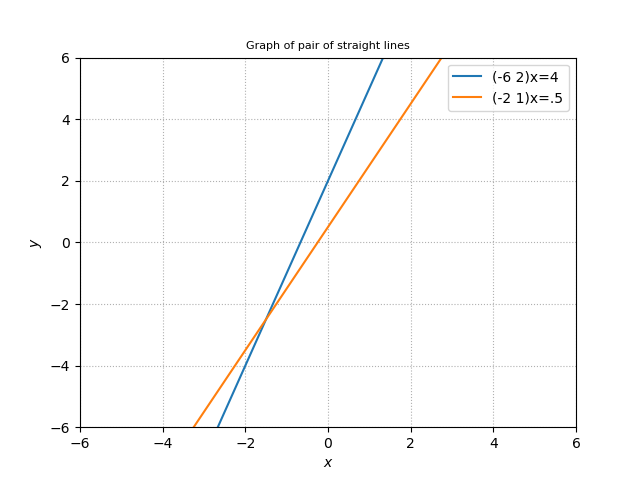
\includegraphics[width=\columnwidth]{Figure.png}
\caption{Pair of lines}
\end{figure}
\begin{comment}
\end{comment}
\end{document}
